\documentclass{beamer}
\usetheme{metropolis}
\beamertemplatetransparentcoveredhigh

\usepackage[portuges]{babel}
\usepackage[utf8]{inputenc}
\usepackage{graphicx}
\graphicspath{{./figs/}}
\usepackage{listings}
\usepackage{color}
\usepackage{hyperref}
\usepackage{xpatch}
\usepackage{comment}
\usepackage[absolute,overlay]{textpos}

\usepackage{tikz}
\usetikzlibrary{calc,shapes.multipart,chains,arrows}

\usepackage[outputdir=build]{minted}
\makeatletter
\AtBeginEnvironment{minted}{\dontdofcolorbox}
\def\dontdofcolorbox{\renewcommand\fcolorbox[4][]{##4}}
\xpatchcmd{\inputminted}{\minted@fvset}{\minted@fvset\dontdofcolorbox}{}{}
\xpatchcmd{\mintinline}{\minted@fvset}{\minted@fvset\dontdofcolorbox}{}{}
\makeatother
\setminted[c]{
  linenos=true,
  breaklines=true,
  encoding=utf8,
  frame=lines,
  framerule=0.5pt,
  autogobble,
  fontsize=\footnotesize,
}
\setminted[bash]{
  linenos=true,
  encoding=utf8,
  frame=lines,
  framerule=0.5pt,
  autogobble,
  fontsize=\small
}
\newcommand{\cod}[1]{\mintinline{c}{#1}}

\definecolor{dkgreen}{rgb}{0,0.6,0}
\definecolor{gray}{rgb}{0.5,0.5,0.5}
\definecolor{mauve}{rgb}{0.58,0,0.82}
\definecolor{uipoppy}{rgb}{225, 64, 5}
\definecolor{uipaleblue}{rgb}{66,58,87}
\definecolor{uiblue}{rgb}{0, 0, 255}
\definecolor{uiblack}{rgb}{0, 0, 0}
\definecolor{uigray}{rgb}{100, 100, 100}
\definecolor{darkgreen}{rgb}{0, 128, 0}

\newcommand{\textcolortwo}[2]{\textcolor{#1}{#2}}
\newcommand{\textgray}[1]{\textcolortwo{uigray}{#1}}
\newcommand{\textpurple}[1]{\textcolortwo{uipaleblue}{#1}}
\newcommand{\textbpurple}[1]{\textbf{\textpurple{#1}}}
\newcommand{\textblue}[1]{\textcolortwo{uiblue}{#1}}
\newcommand{\textbblue}[1]{\textbf{\textblue{#1}}}
\newcommand{\textpoppy}[1]{\textcolortwo{uipoppy}{#1}}
\newcommand{\textbpoppy}[1]{\textbf{\textpoppy{#1}}}
\newcommand{\textred}[1]{\textcolortwo{red}{#1}}
\newcommand{\textbred}[1]{\textbf{\textred{#1}}}
\newcommand{\textgreen}[1]{\textcolortwo{darkgreen}{#1}}
\newcommand{\textbgreen}[1]{\textbf{\textgreen{#1}}}

\definecolor{Purple}{HTML}{911146}
\definecolor{Orange}{HTML}{CF4A30}
\setbeamercolor{alerted text}{fg=Orange}
\setbeamercolor{frametitle}{bg=Purple}
\setbeamercolor{block body}{bg=Purple!20,fg=black}
\setbeamercolor{block title}{bg=Purple!50,fg=black}
\setbeamertemplate{blocks}[rounded][shadow=true]


\newcounter{ExercicioCounter}
\newcommand{\exercicio}{\refstepcounter{ExercicioCounter} Exercício~\theExercicioCounter}

\newcommand\blfootnote[1]{%
  \begingroup
  \renewcommand\thefootnote{}\footnote{#1}%
  \addtocounter{footnote}{-1}%
  \endgroup
}

\newcommand{\setcoverbg}{
  \setbeamertemplate{background}
  {
\includegraphics[width=\paperwidth,height=\paperheight]{backgrounds/coverbg}}
}
\newcommand{\setsectionbg}{
  \setbeamertemplate{background}
  {
\includegraphics[width=\paperwidth,height=\paperheight]{backgrounds/blank}}
}

\setcounter{tocdepth}{4}

\title{Programação Estruturada}
\subtitle{Listas Ligadas}

\author{Professores Emílio Francesquini e Carla Negri Lintzmayer}
\institute{Centro de Matemática, Computação e Cognição\\ Universidade Federal do ABC}
\date{2018.Q3}

\begin{document}

\setcoverbg
\maketitle
\setsectionbg



%%%%%%%%%%%%%%%%%%%%%%%%%%%%%%%%%%%%
\begin{frame}[plain]{Disclaimer}

    \begin{itemize}
        \item Esses slides foram preparados para um curso de Programação Estruturada ministrado na UFABC.
        \item Este material pode ser usado livremente desde que sejam mantidos os créditos dos autores e da instituição.
        \item Muitos dos exemplos apresentados aqui foram retirados de materiais preparados pelos Profs.\ Tomasz Kowaltowski e Orlando Lee da UNICAMP assim como do Prof.\ Paulo Feofiloff do IME-USP.
    \end{itemize}

\end{frame}

%%%%%%%%%%%%%%%%%%%%%%%%%%%%%%%%%%%%%%%%%%%%
%%%%%%%%%%%%%%%%%%%%%%%%%%%%%%%%%%%%%%%%%%%%
%%%%%%%%%%%%%%%%%%%%%%%%%%%%%%%%%%%%%%%%%%%%
%%%%%%%%%%%%%%%%%%%%%%%%%%%%%%%%%%%%%%%%%%%%
%%%%%%%%%%%%%%%%%%%%%%%%%%%%%%%%%%%%%%%%%%%%
%%%%%%%%%%%%%%%%%%%%%%%%%%%%%%%%%%%%%%%%%%%%
\section{Listas ligadas}

%%%%%%%%%%%%%%%%%%%%%%%%%%%%%%%%%%%%
\begin{frame}[fragile]{Lista ligada}

    \begin{itemize}
        \item Uma \textbblue{lista ligada} (= \textbf{lista encadeada} = \emph{\textbf{linked list}}) é uma estrutura de dados para armazenar uma sequência de elementos
        \begin{itemize}
            \item Neste sentido é parecida com o bom e velho vetor
        \end{itemize}
        \item Cada elemento é armazenado em uma \textbblue{célula} (=~\textbf{nó}~=~\textbf{nodo})
        \item Cada célula também armazena o \textbf{endereço do próximo elemento da lista}
    \end{itemize}

    \vspace{2em}
    \begin{center}
        \begin{tikzpicture}[list/.style={rectangle split, rectangle split parts=2, draw, rectangle split horizontal}, >=stealth, start chain]
            % Nodes
            \node[list,on chain] (A) {12};
            \node[list,on chain] (B) {99};
            \node[list,on chain] (C) {37};
            \node[on chain] (D) {NULL};
            % Arestas
            \draw[*->] let \p1 = (A.two), \p2 = (A.center) in (\x1,\y2) -- (B);
            \draw[*->] let \p1 = (B.two), \p2 = (B.center) in (\x1,\y2) -- (C);
            \draw[*->] let \p1 = (C.two), \p2 = (C.center) in (\x1,\y2) -- (D);
        \end{tikzpicture}
    \end{center}
\end{frame}

%%%%%%%%%%%%%%%%%%%%%%%%%%%%%%%%%%%%
\begin{frame}[fragile]{Lista ligada - Estrutura}

    \begin{minted}{c}
        struct reg {
            int conteudo;
            struct reg *prox;
        };
    \end{minted}

    \begin{center}
        \begin{tikzpicture}[list/.style={rectangle split, rectangle split parts=2, draw, rectangle split horizontal}, >=stealth, start chain]
            % Nodes
            \node[list,on chain] (A) {12};
            \node[on chain] (D) {};
            % Arestas
            \draw[*->] let \p1 = (A.two), \p2 = (D.center) in (\x1,\y2) -- (D);
        \end{tikzpicture}
    \end{center}

    É comum criamos um \cod{typedef} para facilitar o uso
    \vspace{-1em}
    \begin{minted}{c}
        typedef struct reg celula;
    \end{minted}

    E então podemos declarar uma célula e um ponteiro para uma célula assim:
    \vspace{-1em}
    \begin{minted}{c}
        celula c;
        celula *p;
    \end{minted}

\end{frame}

%%%%%%%%%%%%%%%%%%%%%%%%%%%%%%%%%%%%
\begin{frame}[fragile]{Listas ligadas - estrutura}
    \begin{itemize}
        \item Se \cod{c} é uma célula então \cod{c.conteudo} é o conteúdo da célula e \cod{c.prox} é o endereço da próxima célula
        \item Se \cod{p} é o endereço de uma célula, então \cod{p->conteudo} é o conteúdo da célula e \cod{p->prox} é o endereço da próxima célula
        \item Se \cod{p} é o endereço da última célula da lista então \cod{p->prox} vale \cod{NULL}
    \end{itemize}

    \begin{center}
        \begin{tikzpicture}[list/.style={rectangle split, rectangle split parts=2, draw, rectangle split horizontal}, >=stealth, start chain]
            % Nodes
            \node[list,on chain] (A) {3};
            \node[list,on chain] (B) {1};
            \node[list,on chain] (C) {4};
            \node[list,on chain] (D) {1};
            \node[list,on chain] (E) {5};
            \node[on chain] (F) {NULL};
            % Arestas
            \draw[*->] let \p1 = (A.two), \p2 = (A.center) in (\x1,\y2) -- (B);
            \draw[*->] let \p1 = (B.two), \p2 = (B.center) in (\x1,\y2) -- (C);
            \draw[*->] let \p1 = (C.two), \p2 = (C.center) in (\x1,\y2) -- (D);
            \draw[*->] let \p1 = (D.two), \p2 = (D.center) in (\x1,\y2) -- (E);
            \draw[*->] let \p1 = (E.two), \p2 = (E.center) in (\x1,\y2) -- (F);
        \end{tikzpicture}
    \end{center}
\end{frame}

%%%%%%%%%%%%%%%%%%%%%%%%%%%%%%%%%%%%
\begin{frame}[fragile]{Listas ligadas - Representando a lista}

    Repare que a definição das células que compõem uma lista ligada é uma \textbblue{definição recursiva}

    \begin{minted}{c}
        struct reg {
            int conteudo;
            struct reg *prox;
        };
    \end{minted}

    \centering
    \begin{tikzpicture}[list/.style={rectangle split, rectangle split parts=2, draw, rectangle split horizontal}, >=stealth, start chain]
        % Nodes
        \node[list,on chain] (A) {3};
        \node[list,on chain] (B) {1};
        \node[list,on chain] (C) {4};
        \node[list,on chain] (D) {1};
        \node[list,on chain] (E) {5};
        \node[on chain] (F) {NULL};
        % Arestas
        \draw[*->] let \p1 = (A.two), \p2 = (A.center) in (\x1,\y2) -- (B);
        \draw[*->] let \p1 = (B.two), \p2 = (B.center) in (\x1,\y2) -- (C);
        \draw[*->] let \p1 = (C.two), \p2 = (C.center) in (\x1,\y2) -- (D);
        \draw[*->] let \p1 = (D.two), \p2 = (D.center) in (\x1,\y2) -- (E);
        \draw[*->] let \p1 = (E.two), \p2 = (E.center) in (\x1,\y2) -- (F);
    \end{tikzpicture}

    Não por acaso, algoritmos que lidam com listas ligadas podem ser expressos recursivamente de maneira natural.
\end{frame}

%%%%%%%%%%%%%%%%%%%%%%%%%%%%%%%%%%%%
\begin{frame}[fragile]{Listas ligadas - Representando a lista}

    Podemos representar a lista através da primeira célula.
    Assim, o endereço da lista ligada é, efetivamente, o endereço da sua primeira célula

    \begin{minted}{c}
        celula *lista;
    \end{minted}

    \centering
    \begin{tikzpicture}[list/.style={rectangle split, rectangle split parts=2, draw, rectangle split horizontal}, >=stealth, start chain]
        % Nodes
        \node[list,on chain] (A) {3};
        \node[list,on chain] (B) {1};
        \node[list,on chain] (C) {4};
        \node[list,on chain] (D) {1};
        \node[list,on chain] (E) {5};
        \node[on chain] (F) {NULL};
        % Arestas
        \draw[*->] let \p1 = (A.two), \p2 = (A.center) in (\x1,\y2) -- (B);
        \draw[*->] let \p1 = (B.two), \p2 = (B.center) in (\x1,\y2) -- (C);
        \draw[*->] let \p1 = (C.two), \p2 = (C.center) in (\x1,\y2) -- (D);
        \draw[*->] let \p1 = (D.two), \p2 = (D.center) in (\x1,\y2) -- (E);
        \draw[*->] let \p1 = (E.two), \p2 = (E.center) in (\x1,\y2) -- (F);
    \end{tikzpicture}

    \begin{block}<only@1>{Pergunta: Como verificar se uma lista está vazia?}
        \begin{minted}[frame=none]{c}
            int lista_vazia(celula *lista) {
                ...
            }
        \end{minted}
    \end{block}

    \begin{block}<only@2>{Pergunta: Como verificar se uma lista está vazia?}
        \begin{minted}[frame=none]{c}
            int lista_vazia(celula *lista) {
                /* equivalente a if (!lista), por quê? */
                if (lista == NULL)
                    return 1;
                else
                    return 0;
            }
        \end{minted}
    \end{block}

    \begin{block}<only@3>{Pergunta: Como verificar se uma lista está vazia?}
        \begin{minted}[frame=none]{c}
                /* Versao super resumida */
                int lista_vazia(celula *lista) {
                    return !lista;
                }
        \end{minted}
    \end{block}

\end{frame}

%%%%%%%%%%%%%%%%%%%%%%%%%%%%%%%%%%%%%%%%%%%%
%%%%%%%%%%%%%%%%%%%%%%%%%%%%%%%%%%%%%%%%%%%%
%%%%%%%%%%%%%%%%%%%%%%%%%%%%%%%%%%%%%%%%%%%%
%%%%%%%%%%%%%%%%%%%%%%%%%%%%%%%%%%%%%%%%%%%%
%%%%%%%%%%%%%%%%%%%%%%%%%%%%%%%%%%%%%%%%%%%%
%%%%%%%%%%%%%%%%%%%%%%%%%%%%%%%%%%%%%%%%%%%%
\section{Manipulando listas ligadas}

%%%%%%%%%%%%%%%%%%%%%%%%%%%%%%%%%%%%
\begin{frame}[fragile]{API}

    \begin{itemize}
        \item A lista ligada é uma das \textbblue{estruturas de dados} mais comuns.
        \item Muitas linguagens de programação oferecem \textbblue{bibliotecas} recheadas com estruturas de dados para os mais diversos usos.
        \item Programas que queira utilizar essas bibliotecas devem seguir um contrato de utilização especificado pela sua \textbblue{API} (\emph{Application Programming Interface}).
        \begin{itemize}
            \item Em C a maneira mais comum é através do uso de arquivos \cod{.h} como, por exemplo o \cod{math.h}.
        \end{itemize}
    \end{itemize}

    Agora que já definimos uma função (\cod{lista_vazia}), quais outras funções seriam interessantes de incluir na API da nossa lista ligada?

\end{frame}

%%%%%%%%%%%%%%%%%%%%%%%%%%%%%%%%%%%%
\begin{frame}[fragile]{Listas ligadas - API}

    \begin{minted}{c}
        struct reg {
            int conteudo;
            struct reg *prox;
        };

        typedef struct reg celula;

        int lista_vazia(celula* lista);
        void imprime_elementos(celula* lista);
        celula* busca_elemento(int elem, celula* lista);
        void insere_elemento(int elem, celula* lista);
        void remove_elemento(celula* lista);
        int busca_e_remove(int elem, celula* lista);
    \end{minted}

\end{frame}

%%%%%%%%%%%%%%%%%%%%%%%%%%%%%%%%%%%%
%%%%%%%%%%%%%%%%%%%%%%%%%%%%%%%%%%%%
%%%%%%%%%%%%%%%%%%%%%%%%%%%%%%%%%%%%
\subsection{Varredura}

%%%%%%%%%%%%%%%%%%%%%%%%%%%%%%%%%%%%
\begin{frame}[fragile]{Varrendo elementos - Versão iterativa}

    \begin{minted}{c}
        struct reg {
            int conteudo;
            struct reg *prox;
        };

        typedef struct reg celula;

        ...

        void imprime_elementos(celula* ll) {
            celula* atual = ll;
            while (atual) {
                printf("%d\n", atual->conteudo);
                atual = atual->prox;
            }
        }
    \end{minted}

\end{frame}

%%%%%%%%%%%%%%%%%%%%%%%%%%%%%%%%%%%%
\begin{frame}[fragile]{Varrendo elementos - Versão recursiva}

    \begin{minted}{c}
        struct reg {
            int conteudo;
            struct reg *prox;
        };
        typedef struct reg celula;

        ...

        void imprime_rec(celula* ll) {
            if (ll) {
                printf("%d\n", ll->conteudo);
                imprime_rec(ll->prox);
            }
        }
\end{minted}

\end{frame}

%%%%%%%%%%%%%%%%%%%%%%%%%%%%%%%%%%%%
\subsubsection{Exercícios}

%%%%%%%%%%%%%%%%%%%%%%%%%%%%%%%%%%%%
\begin{frame}{Exercícios}
    \begin{itemize}
        \item \textbf{\exercicio}~-- Faça uma versão \textbf{iterativa} de \cod{imprime_elementos} que imprime os elementos da lista na ordem inversa.
        \item \textbf{\exercicio}~-- Faça uma versão \textbf{recursiva} de \cod{imprime_elementos} que imprime os elementos da lista na ordem inversa.
    \end{itemize}
\end{frame}

%%%%%%%%%%%%%%%%%%%%%%%%%%%%%%%%%%%%
%%%%%%%%%%%%%%%%%%%%%%%%%%%%%%%%%%%%
%%%%%%%%%%%%%%%%%%%%%%%%%%%%%%%%%%%%
\subsection{Busca}

%%%%%%%%%%%%%%%%%%%%%%%%%%%%%%%%%%%%
\begin{frame}[fragile]{Busca - Versão iterativa}

    \begin{minted}{c}
        struct reg {
            int conteudo;
            struct reg *prox;
        };

        typedef struct reg celula;
        ...

        celula* busca_elemento(int elem, celula* lista) {
            celula* atual = lista;
            while (atual) {
                if (atual->conteudo == elem)
                    return atual;
                atual = atual->prox;
            }
            return NULL;
        }
    \end{minted}

\end{frame}

%%%%%%%%%%%%%%%%%%%%%%%%%%%%%%%%%%%%
\begin{frame}[fragile]{Busca -- Versão recursiva}

    \begin{minted}{c}
        struct reg {
            int conteudo;
            struct reg *prox;
        };

        typedef struct reg celula;

        ...

        celula* busca_elemento_rec(int elem, celula* lista) {
            if (!lista)
                return NULL;
            if (lista->conteudo == elem)
                return lista;
            else
                return busca_elemento_rec(elem, lista->prox);
        }
    \end{minted}

\end{frame}

%%%%%%%%%%%%%%%%%%%%%%%%%%%%%%%%%%%%
%%%%%%%%%%%%%%%%%%%%%%%%%%%%%%%%%%%%
%%%%%%%%%%%%%%%%%%%%%%%%%%%%%%%%%%%%
\subsection{Inserção e remoção}

%%%%%%%%%%%%%%%%%%%%%%%%%%%%%%%%%%%%
\begin{frame}[fragile]{Inserção}

    \begin{minted}{c}
        void insere_elemento(int elem, celula *lista) {
            celula nova;
            nova.conteudo = elem;
            nova.prox = lista->prox;
            lista->prox = &nova;
        }
    \end{minted}

    \only<2>{\begin{textblock*}{20mm}(95mm,40mm)
\includegraphics[width=20mm]{wrong.png}\end{textblock*}}

\end{frame}

%%%%%%%%%%%%%%%%%%%%%%%%%%%%%%%%%%%%
\begin{frame}[fragile]{Inserção}

    \begin{minted}{c}
        void insere_elemento(int elem, celula *inicial) {
            celula *nova;
            nova = malloc(sizeof(celula));
            nova->conteudo = elem;
            nova->prox = inicial;
            inicial = nova;
        }
    \end{minted}

    \begin{onlyenv}<2>
        \begin{minted}{c}
            celula *primeiro;
            int k = 7;
            ...
            /* cria cópia de primeiro */
            insere_elemento(k, primeiro);
        \end{minted}

        Ao voltar da chamada, o valor da variável primeiro \textbf{não foi alterado}.
    \end{onlyenv}
    \only<2>{\begin{textblock*}{20mm}(95mm,25mm)
\includegraphics[width=20mm]{wrong.png}\end{textblock*}}

\end{frame}


%%%%%%%%%%%%%%%%%%%%%%%%%%%%%%%%%%%%
\begin{frame}[fragile]{Remoção}

    \begin{minted}{c}
        /* Remove a célula seguinte à celula apontada por p */
        void remove_elemento(celula *p) {
            celula *removida;
            removida = p->prox;
            p->prox = removida->prox;
            free(removida);
        }
    \end{minted}

    Note que a operação remove a célula seguinte àquela apontada por \cod{p}.

    \pause
    \textbf{Qual o problema disso?}

\end{frame}

%%%%%%%%%%%%%%%%%%%%%%%%%%%%%%%%%%%%
\begin{frame}[fragile]{Problemas com a implementação atual}

    \begin{itemize}
        \item Nossas implementações de inserção e remoção \textbred{não funcionam}!
        \begin{itemize}
            \item \textbf{Como inserir o primeiro} item na lista?
            \item Supondo que já existam itens na lista, \textbf{como remover o primeiro deles}?
        \end{itemize}
    \end{itemize}

\end{frame}

%%%%%%%%%%%%%%%%%%%%%%%%%%%%%%%%%%%%
\begin{frame}[fragile]{Inserção - 1ª tentativa de conserto}

    \begin{minted}{c}
        celula* insere_elemento(int elem, celula* inicial) {
            celula *nova;
            nova = malloc(sizeof(celula));
            nova->conteudo = elem;
            nova->prox = inicial;
            return nova; /* devolve o inı́cio da lista */
        }

        ...
        primeiro = insere_elemento(k, primeiro);
    \end{minted}

    Solução um tanto \textbf{artificial}: fica atualizando o ponteiro para o início sempre.
\end{frame}

%%%%%%%%%%%%%%%%%%%%%%%%%%%%%%%%%%%%
\begin{frame}[fragile]{Inserção - 2ª tentativa de conserto}

    \begin{minted}{c}
        void insere_elemento(int elem, celula** pini) {
            celula *nova;
            nova = malloc(sizeof(celula));
            nova->conteudo = elem;
            nova->prox = *pini;
            *pini = nova;
        }

        ...

        insere_elemento(k, &primeiro);
    \end{minted}

    \begin{itemize}
        \item Um pouco difícil de ler por causa da indireção.
        \item Nenhuma das soluções é satisfatória porque elas diferem do caso geral.
    \end{itemize}

\end{frame}

%%%%%%%%%%%%%%%%%%%%%%%%%%%%%%%%%%%%
\begin{frame}[fragile]{Remoção - Tentativa de conserto}

    \begin{itemize}
        \item Em vez passar como parâmetro o nó anterior, por que não passar o nó que desejamos remover?
        \item \textbf{Isso não é uma boa ideia. Por quê?}
    \end{itemize}

\end{frame}

%%%%%%%%%%%%%%%%%%%%%%%%%%%%%%%%%%%%
\begin{frame}[fragile]{Consertando a inserção e a remoção}

    \begin{itemize}
        \item Temos dois problemas semelhantes: tanto a inserção quanto a remoção não estão muito ``redondas'' no caso do primeiro nó.
        \item \textbf{Como resolver?}
    \end{itemize}

    \only<2>{
        \textbf{Solução:} \textbblue{Listas com cabeças}!
        \begin{textblock*}{40mm}(70mm,50mm)
\includegraphics[width=40mm]{cabeca}\end{textblock*}
    }
\end{frame}

%%%%%%%%%%%%%%%%%%%%%%%%%%%%%%%%%%%%
\begin{frame}[fragile]{Listas com cabeça}

    \centering
    \vspace{1em}
    \begin{tikzpicture}[list/.style={rectangle split, rectangle split parts=2, draw, rectangle split horizontal}, >=stealth, start chain]
        % Nodes
        \node[list,on chain] (E) {};
        \node[list,on chain] (A) {12};
        \node[list,on chain] (B) {99};
        \node[list,on chain] (C) {37};
        % \node[on chain,draw,inner sep=6pt] (D) {}; %NULL
        \node[on chain] (D) {NULL};
        % NULL - X
        % \draw (D.north east) -- (D.south west);
        % \draw (D.north west) -- (D.south east);
        % Arestas
        \draw[*->] let \p1 = (E.two), \p2 = (E.center) in (\x1,\y2) -- (A);
        \draw[*->] let \p1 = (A.two), \p2 = (A.center) in (\x1,\y2) -- (B);
        \draw[*->] let \p1 = (B.two), \p2 = (B.center) in (\x1,\y2) -- (C);
        \draw[*->] let \p1 = (C.two), \p2 = (C.center) in (\x1,\y2) -- (D);
    \end{tikzpicture}

    \begin{textblock*}{15mm}(14mm,11mm)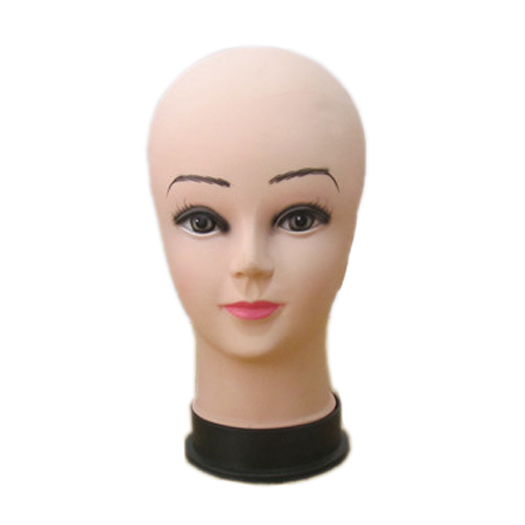
\includegraphics[width=13mm]{cabeca2}\end{textblock*}

    \pause

    \vspace{1em}
    \begin{tikzpicture}[list/.style={rectangle split, rectangle split parts=2, draw, rectangle split horizontal}, >=stealth, start chain]
        % Nodes
        \node[list,on chain] (E) {X};
        \node[list,on chain] (A) {12};
        \node[list,on chain] (B) {99};
        \node[list,on chain] (C) {37};
        % \node[on chain,draw,inner sep=6pt] (D) {}; %NULL
        \node[on chain] (D) {NULL};
        % Arestas
        \draw[*->] let \p1 = (E.two), \p2 = (E.center) in (\x1,\y2) -- (A);
        \draw[*->] let \p1 = (A.two), \p2 = (A.center) in (\x1,\y2) -- (B);
        \draw[*->] let \p1 = (B.two), \p2 = (B.center) in (\x1,\y2) -- (C);
        \draw[*->] let \p1 = (C.two), \p2 = (C.center) in (\x1,\y2) -- (D);
    \end{tikzpicture}

    \begin{itemize}
        \item A \textbblue{cabeça} (=~\textbf{\emph{head}}) da lista ligada serve apenas como um marco de início.
        (Como tal, \textbf{ignoramos} o seu conteúdo.)
        \item Uma lista encadeada \cod{lista} com cabeça está vazia se e somente se \cod{lista->prox == NULL}.
    \end{itemize}

    \begin{minted}[fontsize=\scriptsize]{c}
        /* versão sem cabeça */           /* versão com cabeça */
        int lista_vazia(celula *lst) {    int lista_vazia(celula *lst) {
            return !lst;                      return !lst->prox;
        }                                 }
    \end{minted}

\end{frame}

%%%%%%%%%%%%%%%%%%%%%%%%%%%%%%%%%%%%
\begin{frame}[fragile]{Listas com cabeça}

    Para \textbf{criar} uma lista encadeada vazia com cabeça
    \begin{minted}{c}
        celula *lista;
        lista = malloc(sizeof(celula));
        lista->prox = NULL;
    \end{minted}

    Para \textbf{varrer} (imprimindo) os elementos:
    \begin{minted}{c}
        void imprima(celula *lista) {
            celula *p;
            for (p = lista->prox; p != NULL; p = p->prox)
                printf ("%d\n", p->conteudo);
        }
    \end{minted}

    Como \textbf{adaptar} as demais funções da API?
\end{frame}

%%%%%%%%%%%%%%%%%%%%%%%%%%%%%%%%%%%%
\begin{frame}[fragile]{Manipulando listas com cabeça}

    \begin{itemize}
        \item \textbf{Busca}
            \begin{minted}{c}
                celula* busca_elemento(int elem, celula* lista) {
                    celula* atual = lista->prox; /* lista aponta para a cabeca */
                    while (atual) {
                        if (atual->conteudo == elem)
                            return atual;
                        atual = atual->prox;
                    }
                    return NULL;
                }
            \end{minted}

        \item \textbf{Inserção e remoção}
        \begin{itemize}
            \item Nada muda.
        \end{itemize}
    \end{itemize}

\end{frame}

%%%%%%%%%%%%%%%%%%%%%%%%%%%%%%%%%%%%
\begin{frame}[fragile]{Busca e remoção integradas}

    \begin{minted}{c}
        /* Remove da lista (com cabeça) 'lista' a primeira célula que contém 'elem' */
        void busca_e_remove(int elem, celula* lista) {
            celula *p, *q;
            p = lista;
            q = lista->prox;
            while (q != NULL && q->conteudo != elem) {
                p = q;
                q = q->prox;
            }
            if (q != NULL) {
                p->prox = q->prox;
                free(q);
            }
        }
    \end{minted}

\end{frame}

%%%%%%%%%%%%%%%%%%%%%%%%%%%%%%%%%%%%
\subsubsection{Exercícios}

%%%%%%%%%%%%%%%%%%%%%%%%%%%%%%%%%%%%
\begin{frame}[fragile]{Exercício}
    \textbf{\exercicio}~-- Implemente uma versão semelhante ao \cod{busca_e_remove} que funda as operações de busca e inserção.

    % \begin{minted}{c}
    %     void busca_e_insere (int x, int y, celula* lista) {
    %     celula *p, *q, *nova;
    %     nova = malloc (sizeof (celula));
    %     nova->conteudo = x;
    %     p = lista;
    %     q = lista->prox;
    %     while (q != NULL && q->conteudo != y) {
    %     p = q;
    %     q = q->prox;
    %     }
    %     nova->prox = q;
    %     p->prox = nova;
    %     }
    % \end{minted}
\end{frame}

%%%%%%%%%%%%%%%%%%%%%%%%%%%%%%%%%%%%
%%%%%%%%%%%%%%%%%%%%%%%%%%%%%%%%%%%%
%%%%%%%%%%%%%%%%%%%%%%%%%%%%%%%%%%%%
%%%%%%%%%%%%%%%%%%%%%%%%%%%%%%%%%%%%
%%%%%%%%%%%%%%%%%%%%%%%%%%%%%%%%%%%%
%%%%%%%%%%%%%%%%%%%%%%%%%%%%%%%%%%%%
\section{Vetores ou listas ligadas?}

%%%%%%%%%%%%%%%%%%%%%%%%%%%%%%%%%%%%
\begin{frame}[fragile]{Comparação entre vetores e listas ligadas}

    \textbf{Pergunta:} O que é melhor usar: \textbf{vetores} ou \textbf{listas ligadas}?
    \textbf{Resposta}: Depende.
    \begin{itemize}
        \item Vetores permitem indexação e usar menos memória (não precisa de ponteiros)
        \item Listas ligadas são mais flexíveis
        \begin{itemize}
            \item Não é preciso saber o número de elementos a priori
            \item Algumas operações podem ser mais simples
        \end{itemize}
    \end{itemize}

\end{frame}

%%%%%%%%%%%%%%%%%%%%%%%%%%%%%%%%%%%%
\begin{frame}[fragile]{Comparação entre vetores e listas ligadas}

    \textbf{Exemplo} Suponha que queremos manter um conjunto $S$ de inteiros.
    Devemos ser capazes de realizar as seguintes operações sobre esse conjunto:

    \begin{itemize}
        \item mínimo
        \item $k$-ésimo menor
        \item busca
        \item inserção
        \item remoção
    \end{itemize}

    Considere que $n = |S|$.
\end{frame}

%%%%%%%%%%%%%%%%%%%%%%%%%%%%%%%%%%%%
\begin{frame}[fragile]{Vetores vs. listas ligadas}

    Implementação como um \textbf{vetor ordenado}:
    \begin{itemize}
        \item mínimo: custo $1$
        \item $k$-ésimo menor: custo $1$
        \item busca: custo $\le\log_2n$ (busca binária)
        \item inserção: custo $\le n$ (busca + movimentação de dados)
        \item remoção: custo $\le n$ (busca + movimentação de dados)
    \end{itemize}

    Implementação como uma \textbf{lista ligada ordenada}:
    \begin{itemize}
        \item mínimo: custo $1$
        \item $k$-ésimo menor: custo $k$
        \item busca: custo $\le n$
        \item inserção: custo $\le n$ (busca)
        \item remoção: custo $\le n$ (busca)
    \end{itemize}

\end{frame}



%%%%%%%%%%%%%%%%%%%%%%%%%%%%%%%%%%%%%%%%%%%%
%%%%%%%%%%%%%%%%%%%%%%%%%%%%%%%%%%%%%%%%%%%%
%%%%%%%%%%%%%%%%%%%%%%%%%%%%%%%%%%%%%%%%%%%%
%%%%%%%%%%%%%%%%%%%%%%%%%%%%%%%%%%%%%%%%%%%%
%%%%%%%%%%%%%%%%%%%%%%%%%%%%%%%%%%%%%%%%%%%%
%%%%%%%%%%%%%%%%%%%%%%%%%%%%%%%%%%%%%%%%%%%%
\section{Informações extras - Ordenação}

%%%%%%%%%%%%%%%%%%%%%%%%%%%%%%%%%%%%
\begin{frame}[fragile]{Ordenação}

    Considere a lista ligada definida abaixo:
    \begin{minted}{c}
        struct No {
            int info;
            struct No *prox;
        }

        typedef struct No No;
    \end{minted}

    \begin{itemize}
        \item Vamos descrever três algoritmos para ordenar uma lista ligada com cabeça pelo campo info.
        \item Vocês já conhecem alguns desses algoritmos implementados com vetores!
    \end{itemize}
\end{frame}

%%%%%%%%%%%%%%%%%%%%%%%%%%%%%%%%%%%%%%%%%%%%
%%%%%%%%%%%%%%%%%%%%%%%%%%%%%%%%%%%%%%%%%%%%
%%%%%%%%%%%%%%%%%%%%%%%%%%%%%%%%%%%%%%%%%%%%
\subsection{Ordenação por seleção}

%%%%%%%%%%%%%%%%%%%%%%%%%%%%%%%%%%%%
\begin{frame}[fragile]{Ordenação por seleção}

    \textbblue{Ordenação por seleção} (=\textbf{\emph{selection sort}})
    \begin{itemize}
        \item A ideia básica consiste, em cada iteração:
        \begin{itemize}
            \item \textbf{encontrar e remover} o menor elemento \cod{x} da lista original \cod{ini}
            \item inserir \cod{x} no final de uma lista ordenada formada pelos elementos previamente removidos
        \end{itemize}
        \item Vamos trabalhar usando uma \textbf{lista com cabeça}
    \end{itemize}
\end{frame}

%%%%%%%%%%%%%%%%%%%%%%%%%%%%%%%%%%%%
\begin{frame}[fragile]{Ordenação por seleção}

    \begin{minted}{bash}
    void selectionsort(No *ini) {
        faça t apontar para a lista ini;
        faça ini ser a lista vazia;
        enquanto t for não vazia {
            remova o menor elemento de t;
            insira o elemento no final de ini;
        }
    }
    \end{minted}

    Note que é conveniente ter um ponteiro para o final da lista.
\end{frame}

%%%%%%%%%%%%%%%%%%%%%%%%%%%%%%%%%%%%
\begin{frame}[fragile]{Ordenação por seleção}

    \begin{minted}{c}
        void selectionsort(No *ini) {
            No *t = malloc(sizeof(No)), *last, *min;

            t->prox = ini->prox;
            ini->prox = NULL;
            last = ini;
            while (t->prox != NULL) {
                min = remove_minimo(t);
                last->prox = min;
                last = min;
                last->prox = NULL;
            }
            free(t);
        }
    \end{minted}

\end{frame}

%%%%%%%%%%%%%%%%%%%%%%%%%%%%%%%%%%%%
\begin{frame}[fragile]{Ordenação por seleção}

    \vspace{-1.5em}
    \begin{minted}{c}
       No *remove_minimo(No *ini) {
           No *p, *q, *ant;
           if (!ini->prox)
               return NULL;
           p = ant = ini;
           q = ini->prox;
           while (q) {
               if (q->info < ant->prox->info)
                   ant = p;
               p = q;
               q = q->prox;
           }
           q = ant->prox;
           ant->prox = q->prox;
           return q;
       }
    \end{minted}

    \vspace{-1em}
    Na função, \cod{ant} aponta para o \textbf{nó anterior} ao nó com menor \cod{info} encontrado até o momento.
\end{frame}

%%%%%%%%%%%%%%%%%%%%%%%%%%%%%%%%%%%%
\begin{frame}[fragile]{Ordenação por seleção}

    \begin{minted}{c}
        No *remove_minimo(No *ini) { /* outro jeito */
            No **p, **min, *q;
            if (!ini->prox)
                return NULL;
            p = min = &(ini->prox);
            while (*p) {
                if ((*p)->info < (*min)->info)
                    min = p;
                p = &((*p)->prox);
            }
            q = (*min);
            *min = q->prox;
            return q;
        }
    \end{minted}

    As variáveis \cod{p} e \cod{min} são ponteiros para campos \cod{prox} de nós da lista.
\end{frame}

%%%%%%%%%%%%%%%%%%%%%%%%%%%%%%%%%%%%
\begin{frame}[fragile]{Ordenação por seleção - Análise}

    \begin{itemize}
        \item Podemos analisar a complexidade da função \cod{selectionsort} em função de $n$: o tamanho da lista \cod{ini}
        \item O tempo gasto por \cod{remove_minimo} é proporcional a $n$
        \item \cod{selectionsort} chama \cod{remove_minimo} $n$ vezes
        \item Assim, no total o tempo gasto é \textbf{proporcional a $n^2$}
    \end{itemize}

\end{frame}

%%%%%%%%%%%%%%%%%%%%%%%%%%%%%%%%%%%%
\subsubsection{Exercícios}

%%%%%%%%%%%%%%%%%%%%%%%%%%%%%%%%%%%%
\begin{frame}{Exercício}
    \textbf{\exercicio}~-- É possível simplificar o código apresentado para efetuar a ordenação por seleção de forma que ela coloque o vetor em ordem crescente buscando a célula que contém o máximo da lista e colocando no início da lista de resposta.
    Implemente esta versão supondo que a lista tem cabeça.
\end{frame}

%%%%%%%%%%%%%%%%%%%%%%%%%%%%%%%%%%%%
\begin{frame}[fragile]{Exercício}

    \textbf{\exercicio}~-- Escreva uma versão de \cod{No *selectionsort(No *ini)} que recebe uma lista ligada \textbf{sem cabeça} \cod{ini} e devolve um ponteiro para uma \textbf{lista ligada ordenada sem cabeça} com os nós da lista original.

    \textbf{Sugestão:} em vez de usar uma função \cod{remove_minimo} é melhor escrever o código que faz isto dentro da função \cod{selectionsort}, para evitar o problema de ter de remover um nó no início da lista.
    Não fica tão modularizado, obviamente.
    Outra ideia é usar um ponteiro para ponteiro como parâmetro.
\end{frame}

%%%%%%%%%%%%%%%%%%%%%%%%%%%%%%%%%%%%
%%%%%%%%%%%%%%%%%%%%%%%%%%%%%%%%%%%%
%%%%%%%%%%%%%%%%%%%%%%%%%%%%%%%%%%%%
\subsection{Ordenação por inserção}

%%%%%%%%%%%%%%%%%%%%%%%%%%%%%%%%%%%%
\begin{frame}[fragile]{Ordenação por inserção}
    \textbblue{Ordenação por inserção} (=~\textbf{\emph{insertion sort}})
    \begin{itemize}
        \item A ideia básica consiste, em cada iteração:
        \begin{itemize}
            \item remover o primeiro elemento \cod{x} da lista original \cod{ini}
            \item inserir \cod{x} na posição correta de uma lista ordenada formada pelos elementos previamente removidos
        \end{itemize}
        \item Na implementação em C, passamos o nó cabeça da lista que queremos ordenar e este deve ser o nó cabeça da lista ordenada.
    \end{itemize}
\end{frame}

%%%%%%%%%%%%%%%%%%%%%%%%%%%%%%%%%%%%
\begin{frame}[fragile]{Ordenação por inserção}

    \begin{minted}{bash}
        void insertionsort(No *ini) {
            faça t apontar para a lista ini;
            faça ini ser a lista vazia;
            enquanto t for não vazia {
                remova o primeiro elemento de t;
                insira o elemento em ordem na lista ini;
            }
        }
    \end{minted}

\end{frame}

%%%%%%%%%%%%%%%%%%%%%%%%%%%%%%%%%%%%
\begin{frame}[fragile]{Ordenação por inserção}

    \begin{minted}{c}
        void insertionsort(No *ini) {
            No *t, *x;
            t = ini->prox;
            ini->prox = NULL;
            while (t) {
                x = t;
                t = t->prox;
                insere_ordenado(ini, x);
            }
        }
    \end{minted}

    A lista \cod{t} não tem cabeça.
\end{frame}

%%%%%%%%%%%%%%%%%%%%%%%%%%%%%%%%%%%%
\begin{frame}[fragile]{Ordenação por inserção}

    \begin{minted}{c}
        void insere_ordenado(No *ini, No *x) {
            No *p, *q,
            p = ini;
            q = ini->prox;
            while (q && q->info < x->info) {
                p = q;
                q = q->prox;
            }
            x->prox = q;
            p->prox = x;
        }
    \end{minted}

\end{frame}

%%%%%%%%%%%%%%%%%%%%%%%%%%%%%%%%%%%%
\begin{frame}[fragile]{Ordenação por inserção -- Análise}

    \begin{itemize}
        \item Podemos analisar a complexidade da função \cod{insertionsort} em função de $n$, o tamanho da lista \cod{ini}.
        \item O tempo gasto por \cod{insere_ordenado} é proporcional a $n$ no pior caso.
        \item \cod{insertionsort} chama \cod{insere_ordenado} $n$ vezes.
        \item Assim, no total o tempo gasto \textbf{é proporcional a no máximo $n^2$}.
    \end{itemize}

\end{frame}


%%%%%%%%%%%%%%%%%%%%%%%%%%%%%%%%%%%%
\subsubsection{Exercícios}

%%%%%%%%%%%%%%%%%%%%%%%%%%%%%%%%%%%%
\begin{frame}{Exercício}
    \textbf{\exercicio}~-- Escreva uma versão de \cod{insere_ordenado} que usa ponteiros para ponteiros (como na segunda versão de \cod{remove_minimo}).
\end{frame}

%%%%%%%%%%%%%%%%%%%%%%%%%%%%%%%%%%%%
%%%%%%%%%%%%%%%%%%%%%%%%%%%%%%%%%%%%
%%%%%%%%%%%%%%%%%%%%%%%%%%%%%%%%%%%%
\subsection{Ordenação por intercalação -- MergeSort}

%%%%%%%%%%%%%%%%%%%%%%%%%%%%%%%%%%%%
\begin{frame}[fragile]{Intercalando duas listas}

    \textbf{Problema:} intercalar (=~\textbf{\emph{merge}}) duas listas ordenadas

    \vspace{2em}

    Queremos implementar a seguinte função:

    \begin{minted}[frame=none,linenos=false]{c}
        No *intercala(No *s, No *t);
    \end{minted}

    A função \cod{intercala} recebe duas \textbf{listas ligadas ordenadas sem cabeça} \cod{s} e \cod{t}, e devolve uma \textbf{lista ordenada sem cabeça} contendo os nós das listas \cod{s} e \cod{t}.

    Também podemos usar listas com cabeça: o código é praticamente idêntico.
    Só é preciso descartar (\cod{free}) uma das cabeças ao final.

\end{frame}

%%%%%%%%%%%%%%%%%%%%%%%%%%%%%%%%%%%%
\begin{frame}[fragile]
    % \vspace{-1.5em}
    \begin{minted}[fontsize=\scriptsize]{c}
        No *intercala(No *s, No *t) {
            No *p, *q, cabeca, *last;
            last = &cabeca;
            cabeca.prox = NULL;
            p = s;
            q = t;
            while (p && q) {
                if (p->info < q->info) {
                    last->prox = p;
                    last = p;
                    p = p->prox;
                } else {
                    last->prox = q;
                    last = q;
                    q = q->prox;
                }
            }
            if (p)
                last->prox = p;
            else
                last->prox = q;
            return cabeca.prox;
        }
    \end{minted}
\end{frame}

%%%%%%%%%%%%%%%%%%%%%%%%%%%%%%%%%%%%
\begin{frame}[fragile]{Mergesort}
    A ideia do algoritmo implementado pela função \cod{mergesort} é conceitualmente muito simples.
    \begin{itemize}
        \item Se a lista \textblue{ini} for pequena, então ordene diretamente.
        \item Caso contrário, divida a lista \cod{ini} em duas listas \cod{s} e \cod{t} de tamanhos aproximadamente iguais.
        \item Recursivamente, ordene as listas \cod{s} e \cod{t}.
        \item Intercale as listas \cod{s} e \cod{t} e devolva a lista resultante.
    \end{itemize}
\end{frame}

%%%%%%%%%%%%%%%%%%%%%%%%%%%%%%%%%%%%
\begin{frame}[fragile]{Mergesort}
    \begin{minted}{c}
        No *mergesort(No *ini) {
            No *met, *metade;
            /* caso base */
            if (ini == NULL || ini->prox == NULL)
                return ini;
            metade = acha_metade(ini);
            met = metade->prox;
            metade->prox = NULL; /* divide a lista */
            ini = mergesort(ini);
            met = mergesort(met);
            return intercala(ini, met);
        }
    \end{minted}
\end{frame}

%%%%%%%%%%%%%%%%%%%%%%%%%%%%%%%%%%%%
\begin{frame}[fragile]{Mergesort}
    \textbf{Como achar a metade rapidamente?}

    \begin{minted}{c}
        No *acha_metade(No *ini) {
            No *slow, *fast;
            if (ini == NULL)
                return ini;
            slow = fast = ini;
            while (fast->prox && fast->prox->prox) {
                slow = slow->prox;
                fast = fast->prox->prox;
            }
            return slow;
        }
    \end{minted}
\end{frame}

%%%%%%%%%%%%%%%%%%%%%%%%%%%%%%%%%%%%
%%%%%%%%%%%%%%%%%%%%%%%%%%%%%%%%%%%%
%%%%%%%%%%%%%%%%%%%%%%%%%%%%%%%%%%%%
\subsubsection{Informações extras: análise (informal) do Mergesort}

%%%%%%%%%%%%%%%%%%%%%%%%%%%%%%%%%%%%
\begin{frame}[fragile]{Mergesort - Análise (informal)}

    Suponha que $T(n)$ seja o tempo de pior caso que o \cod{mergesort} leva para ordenar uma lista ligada com $n$ nós.

    \begin{itemize}
        \item Se $n \ge 2$ então acontecem os seguintes passos:
        \begin{itemize}
            \item Divide a lista
            \item Duas chamadas recursivas
            \item Intercalação
        \end{itemize}

        \item Logo o tempo gasto é:
        \[T(n) = n + 2T(n/2) + n = 2T(n/2) + 2n \]

        \item Assim,
        \[
            T (n) =
            \begin{cases}
                2T (n/2) + 2n, & \text{se } n \geq 2\\
                1,             & \text{caso contrário}

            \end{cases}
        \]
    \end{itemize}
\end{frame}

%%%%%%%%%%%%%%%%%%%%%%%%%%%%%%%%%%%%
\begin{frame}[fragile]{Mergesort - Análise (informal)}

    Para ter uma intuição, suponha que $n = 2^k$. Note que há:
    \begin{itemize}
        \item $1$ chamada para uma lista de tamanho $n$ (\textbf{nível $1$})
        \item $2$ chamadas para uma lista de tamanho $n/2$ (\textbf{nível $2$})
        \item $4$ chamadas para uma lista de tamanho $n/4$ (\textbf{nível $3$})
        \item $2^{i-1}$ chamadas para uma lista de tamanho $n/2^{i-1}$ (\textbf{nível $i$})
        \item $2^k-1$ chamadas para uma lista de tamanho $2$ (\textbf{nível $k - 1$})
        \item $2^k$ chamadas para uma lista de tamanho $1$ (\textbf{nível $k$})
    \end{itemize}

\end{frame}

%%%%%%%%%%%%%%%%%%%%%%%%%%%%%%%%%%%%
\begin{frame}[fragile]{Mergesort - Análise (informal)}

    Ignore o tempo de dividir a lista. Vamos contar o custo das intercalações de listas (IL) em cada nível.
    \begin{itemize}
        \item \textbf{nível $1$}: $1$ IL de tamanho $n/2$; tempo $2 \times (n/2) = n$
        \item \textbf{nível $2$}: $2$ ILs de tamanho $n/4$; tempo $2 \times 2 \times (n/4) = n$
        \item \textbf{nível $3$}: $4$ ILs de tamanho $n/8$; tempo $2 \times 4 \times (n/8) = n$
        \item \textbf{nível $i$}: $2^{i-1}$ ILs de tamanho $n/2^i$ ; tempo $2 \times 2^{i-1}\times (n/2^i) = n$
        \item \textbf{nível $k - 1$}: $2^{k- 2}$ ILs de tamanho 2; tempo $2 \times 2^{k-2}\times(2) = n$
        \item \textbf{nível $k$}: $2^{k-1}$ ILs de tamanho 1; tempo $2 \times 2^{k- 1}\times (1) = n$
    \end{itemize}

    Assim, o tempo total é $(k - 1)n \approx n\log_2n$.

\end{frame}

%%%%%%%%%%%%%%%%%%%%%%%%%%%%%%%%%%%%
\begin{frame}[fragile]{Mergesort - Análise (informal)}

    \begin{itemize}
        \item Para $n$ grande, temos que $n\log_2n << n^2$.
        \item Assim, o algoritmo \cod{mergesort} é bem mais eficiente que os algoritmos quadráticos \cod{bubblesort}, \cod{selectionsort} e \cod{insertionsort}.
    \end{itemize}

\end{frame}

%%%%%%%%%%%%%%%%%%%%%%%%%%%%%%%%%%%%
%%%%%%%%%%%%%%%%%%%%%%%%%%%%%%%%%%%%
\subsubsection{Exercícios}

%%%%%%%%%%%%%%%%%%%%%%%%%%%%%%%%%%%%
\begin{frame}[fragile]{Exercício}
    \textbf{\exercicio}~-- Escreva uma versão \textbf{recursiva} da função \cod{No *intercala(No *s, No *t)} que não use laços.
\end{frame}

%%%%%%%%%%%%%%%%%%%%%%%%%%%%%%%%%%%%
%%%%%%%%%%%%%%%%%%%%%%%%%%%%%%%%%%%%
%%%%%%%%%%%%%%%%%%%%%%%%%%%%%%%%%%%%
%%%%%%%%%%%%%%%%%%%%%%%%%%%%%%%%%%%%
%%%%%%%%%%%%%%%%%%%%%%%%%%%%%%%%%%%%
%%%%%%%%%%%%%%%%%%%%%%%%%%%%%%%%%%%%
\section{Informações extras: listas duplamente ligadas}

%%%%%%%%%%%%%%%%%%%%%%%%%%%%%%%%%%%%
\begin{frame}[fragile]{Listas duplamente ligadas}

    \begin{minted}{c}
        struct NoDuplo {
            int info;
            struct NoDuplo *ant;
            struct NoDuplo *prox;
        };
        typedef struct NoDuplo NoD;
    \end{minted}

    \textbf{Vantagens:} maior acessibilidade

    \textbf{Desvantagens:} dobro de ponteiros e mais trabalho para manter a lista.

\end{frame}

%%%%%%%%%%%%%%%%%%%%%%%%%%%%%%%%%%%%
%%%%%%%%%%%%%%%%%%%%%%%%%%%%%%%%%%%%
%%%%%%%%%%%%%%%%%%%%%%%%%%%%%%%%%%%%
\subsection{Busca}

%%%%%%%%%%%%%%%%%%%%%%%%%%%%%%%%%%%%
\begin{frame}[fragile]{Busca}

    A função \cod{busca} recebe uma lista duplamente ligada \cod{ini} e um inteiro \cod{k}, e devolve um ponteiro para o primeiro nó com chave \cod{k} ou \cod{NULL}, se não houver.

    \begin{minted}{c}
        No *busca(NoD *ini, int k) {
            NoD *p = ini;
            while (p && p->info != k)
                p = p->prox;
            return p;
        }
    \end{minted}

    Virtualmente idêntica à função busca para lista ligadas simples.
\end{frame}

%%%%%%%%%%%%%%%%%%%%%%%%%%%%%%%%%%%%
\begin{frame}[fragile]{Inserção}

    A função \cod{insere} recebe uma lista duplamente ligada \cod{ini} e um elemento \cod{k} e insere um novo nó com conteúdo \cod{k} entre o nó apontado por \cod{p} e o seguinte.
    Só faz sentido se \cod{p != NULL}.

    \begin{minted}{c}
        void insere(NoD *p, int k) {
            NoD *novo;
            novo = malloc(sizeof(NoD));
            novo->info = k;
            novo->prox = p->prox;
            novo->ant = p;
            if (p->prox)
                p->prox->ant = novo;
            p->prox = novo;
        }
    \end{minted}

    Não faz inserção no início de uma lista duplamente ligada, a não ser que tenha nó cabeça.
\end{frame}

%%%%%%%%%%%%%%%%%%%%%%%%%%%%%%%%%%%%
\begin{frame}[fragile]{Remoção}

    A função \cod{remove} recebe um ponteiro \cod{q} para um nó de uma lista duplamente ligada e o remove.

    \begin{minted}{c}
        void remove(NoD *q) {
            No *p = q->ant;
            p->prox = q->prox;
            if (q->prox)
                q->prox->ant = p;
            free(q);
        }
    \end{minted}

    Note a diferença com listas ligadas simples.

    Não funciona se \cod{q} aponta para o primeiro elemento da lista, a não ser que tenha nó cabeça.
\end{frame}

%%%%%%%%%%%%%%%%%%%%%%%%%%%%%%%%%%%%
%%%%%%%%%%%%%%%%%%%%%%%%%%%%%%%%%%%%
%%%%%%%%%%%%%%%%%%%%%%%%%%%%%%%%%%%%
%%%%%%%%%%%%%%%%%%%%%%%%%%%%%%%%%%%%
%%%%%%%%%%%%%%%%%%%%%%%%%%%%%%%%%%%%
%%%%%%%%%%%%%%%%%%%%%%%%%%%%%%%%%%%%
\section{Informações extras: listas ligadas circulares}

%%%%%%%%%%%%%%%%%%%%%%%%%%%%%%%%%%%%
\begin{frame}[fragile]{Listas ligadas circulares}

    Tem a mesma declaração de uma lista ligada simples, mas o campo \cod{prox} do último nó \cod{aponta} para o \cod{primeiro} nó.

    \begin{itemize}
        \item \textbf{Lista ligada circular sem cabeça}: um problema é a lista vazia.
        \item \textbf{Lista ligada circular com cabeça \cod{ini}}
        \begin{itemize}
            \item \textbf{Lista vazia}: \cod{ini->prox == ini}
        \end{itemize}
    \end{itemize}

    Pode-se implementar outras variantes:
    \begin{itemize}
        \item listas ligadas circulares com ou sem cabeça
        \item listas duplamente ligadas circulares
        \item ou com ambas as formas.
    \end{itemize}

\end{frame}

%%%%%%%%%%%%%%%%%%%%%%%%%%%%%%%%%%%%
%%%%%%%%%%%%%%%%%%%%%%%%%%%%%%%%%%%%
%%%%%%%%%%%%%%%%%%%%%%%%%%%%%%%%%%%%
\subsection{Busca}

%%%%%%%%%%%%%%%%%%%%%%%%%%%%%%%%%%%%
\begin{frame}[fragile]{Busca em lista circular}

    A função busca recebe uma lista ligada circular com cabeça \cod{ini} e um inteiro \cod{k}, e devolve um ponteiro para o primeiro nó com chave \cod{k} ou \cod{NULL}, se não houver.

    \begin{minted}{c}
        No *busca(No *ini, int k) {
            No *p = ini->prox;
            ini->info = k; /* sentinela */
            while (p->info != k)
                p = p->prox;
            ini->info = NULL;
            if (p == ini)
                return NULL;
            else
                return p;
        }
    \end{minted}

\end{frame}

%%%%%%%%%%%%%%%%%%%%%%%%%%%%%%%%%%%%
%%%%%%%%%%%%%%%%%%%%%%%%%%%%%%%%%%%%
%%%%%%%%%%%%%%%%%%%%%%%%%%%%%%%%%%%%
\subsection{Exercícios}

%%%%%%%%%%%%%%%%%%%%%%%%%%%%%%%%%%%%
\begin{frame}[fragile]{Exercícios}
    \textbf{\exercicio}~-- Escreva uma função \cod{remove_llcc(No *ini, int k)} que recebe um ponteiro para uma lista ligada circular com cabeça \cod{ini} e remove o primeiro nó com chave \cod{k}.

    \textbf{\exercicio}~-- Escreva uma função \cod{remove_ldlcc(NoD *p)} que recebe um ponteiro para um nó \cod{p} de uma lista duplamente ligada circular com nó cabeça e o remove da lista.
    Naturalmente, suponha que \cod{p} não é o nó cabeça da lista.

    \textbf{\exercicio}~-- Escreva uma função \cod{insere_lcco(No *ini, int k)} que recebe uma lista ligada circular com cabeça ordenada \cod{ini} e insere um novo nó com chave \cod{k} na posição correta.
\end{frame}

%%%%%%%%%%%%%%%%%%%%%%%%%%%%%%%%%%%%
\begin{frame}[fragile]{Exercício: representando polinômios}

    \vspace{-5em}
    Considere o polinômio:\\
    \[P(x) = a_n x^n + a_{n-1} x^{n-1} + ... + a_2 x^2 + a_1 x + a_0\]

    onde $a_n\neq0$

    Representação de \textblue{$P_1(x) = 5x^{10} - 3x^5 + 4$} e \textred{$P_2(x) = 0$}
    \begin{textblock*}{40mm}(10mm,60mm)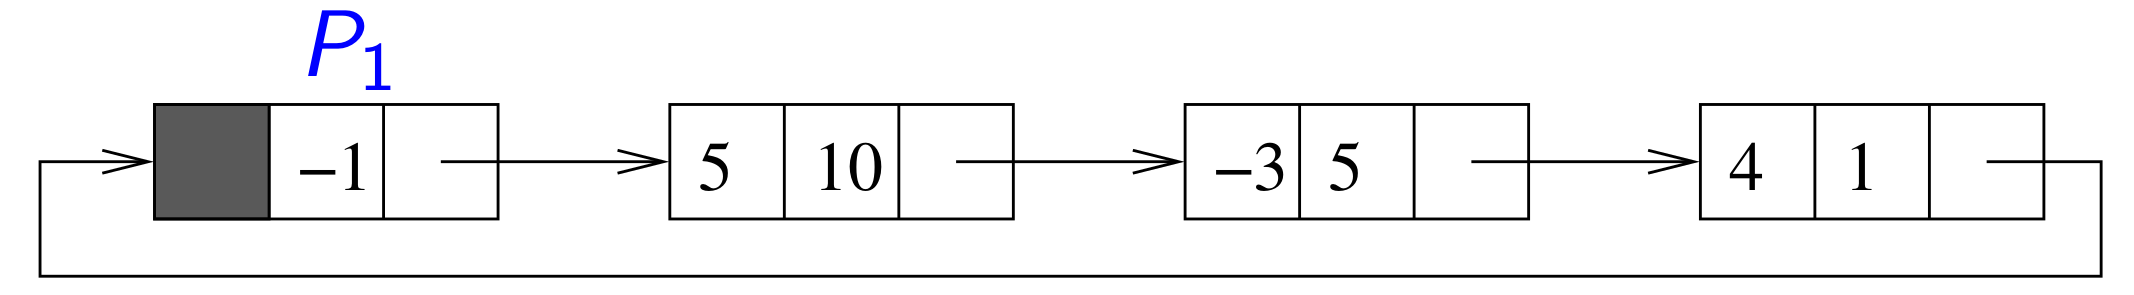
\includegraphics[height=4em]{pum}\end{textblock*}
    \begin{textblock*}{40mm}(48mm,75mm)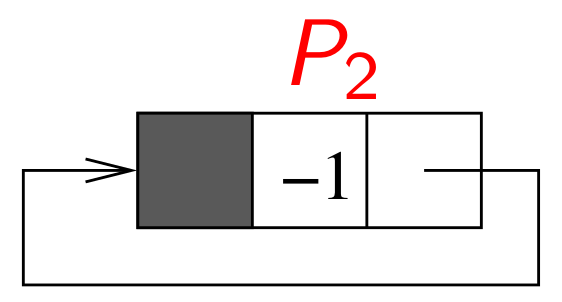
\includegraphics[height=4em]{pdois}\end{textblock*}

\end{frame}

%%%%%%%%%%%%%%%%%%%%%%%%%%%%%%%%%%%%
\begin{frame}[fragile]{Exercício: representando polinômios}

    \begin{minted}{c}
        typedef struct AuxPol {
            float coef;
            int expo;
            struct AuxPol *prox;
        } Termo, *Polin;
    \end{minted}

    A lista tem cabeça. O campo \cod{expo} da cabeça é igual a $-1$ para
    ser usado como sentinela.

    Note que:
    \begin{minted}{c}
        Termo *p;
        Polin p;
    \end{minted}
    são declarações \textbf{equivalentes}.

\end{frame}

%%%%%%%%%%%%%%%%%%%%%%%%%%%%%%%%%%%%
\begin{frame}[fragile]{Exercício: representando polinômios}

    A função \cod{imprime(Polin p)} imprime um polinômio \cod{p} exibindo os pares (\cod{coef}, \cod{expo}) de cada termo.

    \begin{minted}{c}
        void imprime(Polin pol) {
            Termo *p = pol->prox;
            if (p == pol) {
                printf("Polinomio nulo.\n");
                return;
            }
            while (p->expo != -1) {
                printf("%5.1f, %2d ", p->coef, p->expo);
                p = p->prox;
            }
            printf("\n");
        }
    \end{minted}

\end{frame}

%%%%%%%%%%%%%%%%%%%%%%%%%%%%%%%%%%%%
\begin{frame}[fragile]{Exercício: representando polinômios}

    \textbf{\exercicio}~-- Implemente em C funções para cada uma das operações abaixo:
    \begin{itemize}
        \item Calcule o valor de um polinômio $P(x)$ em um ponto $x_0$
        \item Calcule a soma de dois polinômios (usando o método da intercalação)
        \item Calcule o produto de dois polinômios
        \item Calcule a $k$-ésima derivada de um polinômio
    \end{itemize}

\end{frame}

%%%%%%%%%%%%%%%%%%%%%%%%%%%%%%%%%%%%
\begin{frame}[fragile]{Exercício: Problema de Josephus}

    \begin{itemize}
        \item Um grupo de $N$ pessoas precisa eleger um líder.
        \item Decidiu-se usar a seguinte ideia para eleger um líder: forma-se um círculo com as $N$ pessoas e escolhe-se um inteiro $k$.
        Começamos com uma pessoa qualquer e percorremos o círculo em sentido horário, eliminando cada $k$-ésima pessoa.
        A \textbf{última pessoa} que restar será o líder.
        Veja o verbete sobre Josephus na Wikipedia.
    \end{itemize}

    \textbf{Problema de Josephus}: coloque os números $1, 2,\ldots,N$ em um círculo nesta ordem e começando em $1$ aplique o algoritmo acima com um valor $k$.
    Determine o último número, denotado $J(N, k)$.

    \textbf{\exercicio}~-- Escreva uma função \cod{int josephus(int N, int k)} que calcula $J(N, k)$.

\end{frame}

\end{document}
